l%%%%%%%%%%%%%%%%%%%%%%%%%%%%%%%%%%%%%%%%%%%%%%%%%%%%%%%%%%%%%%%%%%%%%%%%%
% KHAI BÁO CÁC THÔNG SỐ ĐỀ THI - MÃ ĐỀ 132
%%%%%%%%%%%%%%%%%%%%%%%%%%%%%%%%%%%%%%%%%%%%%%%%%%%%%%%%%%%%%%%%%%%%%%%%%
\def\toanlop{10}
\def\thoigian{45}
\def\namhoc{2024 - 2025}
\begin{dethi}
	{SỞ GD\&ĐT THỪA THIÊN HUẾ}
	{TRƯỜNG THPT NGUYỄN TRƯỜNG TỘ}
	{KIỂM TRA GIỮA KÌ I}
	{Thời gian làm bài: 45 phút, không kể thời gian phát đề}
\end{dethi}

\Opensolutionfile{ans}[ans/ansTN-NguyenTruongTo102]

\noindent \textbf{PHẦN I. Câu trắc nghiệm nhiều phương án lựa chọn (12 câu = 3 điểm)}

\noindent \textit{(Thí sinh trả lời từ câu 1 đến câu 12. Mỗi câu hỏi thí sinh chỉ chọn một phương án.)}
\vspace{0.2cm}

\begin{ex}%[10V1-102-01]
	Công thức tính vận tốc của chuyển động thẳng biến đổi đều là $v=v_{0}+at$. Đối với chuyển động thẳng nhanh dần đều thì ta luôn có thuộc tính nào dưới đây?
	\choice
	{$v$ luôn dương}
	{$a$ luôn dương}
	{\True $a$ luôn cùng dấu với $v$}
	{$a$ luôn ngược dấu với $v$}
	\loigiai{
		Theo đặc điểm của chuyển động thẳng nhanh dần đều, tốc độ của vật tăng dần theo thời gian, do đó tích số giữa vận tốc và gia tốc luôn dương ($a \cdot v > 0$), nghĩa là vectơ gia tốc $\vec{a}$ luôn cùng dấu với vectơ vận tốc $\vec{v}$. Chọn C.
	}
\end{ex}

\begin{ex}%[10V1-102-02]
	Đâu \textbf{không} phải là một trong các tính chất đặc trưng của vectơ vận tốc của một chất điểm?
	\choice
	{Gốc của vectơ nằm ngay trên chất điểm chuyển động}
	{Có phương trùng với phương chuyển động của chất điểm}
	{\True Có chiều luôn ngược với chiều chuyển động của chất điểm}
	{Độ dài của vectơ tỉ lệ thuận với độ lớn (tốc độ) của vận tốc}
	\loigiai{
		Vectơ vận tốc $\vec{v}$ luôn có chiều hướng trùng khít với chiều chuyển động tức thời của chất điểm, phát biểu khẳng định "ngược chiều chuyển động" là sai. Chọn C.
	}
\end{ex}

\begin{ex}%[10V1-102-03]
	Chọn phát biểu đúng khi nói về thuộc tính đặc trưng của đại lượng quãng đường đi được của một vật?
	\choice
	{\True Quãng đường là một đại lượng vô hướng luôn nhận giá trị không âm}
	{Quãng đường luôn luôn nhận giá trị âm đại số}
	{Quãng đường là một đại lượng vectơ xác định hướng chuyển động}
	{Quãng đường có thể nhận giá trị âm hoặc dương tùy thuộc vào chiều chọn}
	\loigiai{
		Quãng đường đi được $s$ là tổng độ dài của các đoạn quỹ đạo mà vật đã thực hiện vượt qua, do đó nó là một đại lượng vô hướng và luôn nhận giá trị không âm ($s \ge 0$). Chọn A.
	}
\end{ex}

\begin{ex}%[10V1-102-04]
	Gọi $\overline{A}$ là giá trị trung bình, $\Delta A'$ là sai số dụng cụ, $\overline{\Delta A}$ là sai số ngẫu nhiên tuyệt đối. Công thức tính sai số tuyệt đối toàn phần $\Delta A$ của phép đo là
	\choice
	{\True $\Delta A = \overline{\Delta A} + \Delta A'$}
	{$\Delta A = \overline{\Delta A} - \Delta A'$}
	{$\Delta A = \overline{\Delta A} \cdot \Delta A'$}
	{$\Delta A = \overline{\Delta A} / \Delta A'$}
	\loigiai{
		Sai số tuyệt đối toàn phần của một phép đo trực tiếp bằng tổng đại số của sai số ngẫu nhiên trung bình và sai số dụng cụ: $\Delta A = \overline{\Delta A} + \Delta A'$. Chọn A.
	}
\end{ex}

\begin{ex}%[10V1-102-05]
	Một vật chuyển động trên đoạn thẳng, tại một thời điểm vật có vận tốc đại số $v$ và gia tốc đại số $a$. Chuyển động của vật được coi là chậm dần đều khi
	\choice
	{gia tốc $a$ mang giá trị âm}
	{gia tốc $a$ mang giá trị dương}
	{\True tích số $a \cdot v < 0$}
	{vận tốc $v$ mang giá trị âm}
	\loigiai{
		Chuyển động thẳng biến đổi đều được phân loại là chuyển động chậm dần đều khi vectơ gia tốc ngược chiều với vectơ vận tốc tức thời, tương ứng tích số giữa hai giá trị đại số mang dấu âm: $a \cdot v < 0$. Chọn C.
	}
\end{ex}

\begin{ex}%[10V1-102-06]
	Những phân ngành nào sau đây thuộc về đối tượng và lĩnh vực nghiên cứu chính của khoa học Vật lí?
	\choice
	{Cơ học, nhiệt học, cấu trúc tiến hóa của vật chất vô cơ}
	{Nhiệt học, quang học, cơ chế di truyền của sinh vật học}
	{\True Cơ học, nhiệt học, điện học, quang học}
	{Điện học, quang học, thuộc tính hữu cơ của hợp chất}
	\loigiai{
		Cơ học, nhiệt học, điện học và quang học là bốn phân ngành nền tảng cốt lõi nhất cấu thành nên lâu đài Vật lí học cổ điển. Sinh vật học hay vật chất hữu cơ thuộc phạm vi của Sinh học và Hóa học. Chọn C.
	}
\end{ex}

\begin{ex}%[10V1-102-07]
	Biển báo dùng để cảnh báo nguy cơ gây ô nhiễm nguy hiểm chất độc đối với môi trường sinh thái xung quanh là
% TODO: \usepackage{graphicx} required
\begin{center}
	\includegraphics[scale=0.7]{HINHVE-phai-Tikz/VL10-GHKI-NTT-2526-hinh1}
\end{center}
	\choice
	{hình 1 (Biển cảnh báo chất độc sức khỏe)}
	{hình 2 (Biển cảnh báo chất ăn mòn)}
	{hình 3 (Biển cảnh báo nguy cơ điện giật)}
	{\True hình 4 (Biển chứa hình ảnh cá chết và cây khô). }
	\loigiai{
		Biển báo chứa hình ảnh tượng hình cây khô trơ trụi và con cá chết nằm ngửa là kí hiệu cảnh báo tiêu chuẩn quốc tế dùng để chỉ chất độc nguy hại đối với môi trường sinh thái. Chọn D.
	}
\end{ex}

\begin{ex}%[10V1-102-08]
	Một người tập thể dục chạy bộ dọc theo một đường thẳng, trong khoảng thời gian $10\text{ s}$ người đó chạy được quãng đường dài $150\text{ m}$. Tốc độ trung bình trên cả quãng đường chạy của người đó là
	\choice
	{$150\text{ m/s}$}
	{$0,015\text{ m/s}$}
	{\True $15\text{ m/s}$}
	{$15\text{ km/s}$}
	\loigiai{
		Tốc độ trung bình của người chạy bộ xác định theo thương số quãng đường:
		$$v_{\text{tb}} = \frac{s}{t} = \frac{150\text{ m}}{10\text{ s}} = 15\text{ m/s} \text{}$$
		Chọn C.
	}
\end{ex}

\begin{ex}%[10V1-102-09]
	Một người đi xe máy đang chuyển động thẳng đều thì tài xế thực hiện hãm phanh để giảm tốc độ cho xe dừng lại ở đích. Nếu chọn chiều dương hướng trùng với chiều chuyển động của xe, nhận xét nào sau đây đúng về dấu của các đại lượng?
	\choice
	{$a > 0, v > 0$}
	{$a < 0, v < 0$}
	{$a > 0, v < 0$}
	{\True $a < 0, v > 0$}
	\loigiai{
		- Vì xe máy chuyển động theo chiều dương nên vận tốc tức thời mang giá trị dương: $v > 0$. \\
		- Hành động hãm phanh làm tốc độ giảm đặc trưng cho chuyển động chậm dần đều, pít-tông gia tốc phải hướng ngược chiều chuyển động (ngược chiều dương) nên nhận giá trị âm: $a < 0$. Chọn D.
	}
\end{ex}

\begin{ex}%[10V1-102-10]
	Nếu chọn mốc thời gian xuất phát của một chuyển động là lúc $t_{0}=8\text{ h}$ và tổng thời gian chuyển động thực tế kéo dài trong $3\text{ h}$ thì thời điểm kết thúc hành trình chuyển động là lúc
	\choice
	{$8\text{ h}$}
	{$10\text{ h}$}
	{\True $11\text{ h}$}
	{$12\text{ h}$}
	\loigiai{
		Thời điểm kết thúc hành trình bằng tổng số giữa thời điểm chọn làm mốc ban đầu và khoảng thời gian chuyển động: $t = t_0 + \Delta t = 8\text{ h} + 3\text{ h} = 11\text{ h}$. Chọn C.
	}
\end{ex}

\begin{ex}%[10V1-102-11]
	Đồ thị độ dịch chuyển – thời gian $(d-t)$ của một xe chuyển động thẳng có dạng đường thẳng dốc xuống từ vạch $80\text{ km}$ về vạch $0\text{ km}$ kéo dài trong khoảng thời gian $2\text{ h}$ như đường (2) ở hình vẽ. Ta kết luận vật đang chuyển động như thế nào?
	% TODO: \usepackage{graphicx} required
% TODO: \usepackage{graphicx} required
\begin{center}
	\includegraphics[scale=1]{HINHVE-phai-Tikz/VL10-GHKI-NTT-2526-hinh2}
	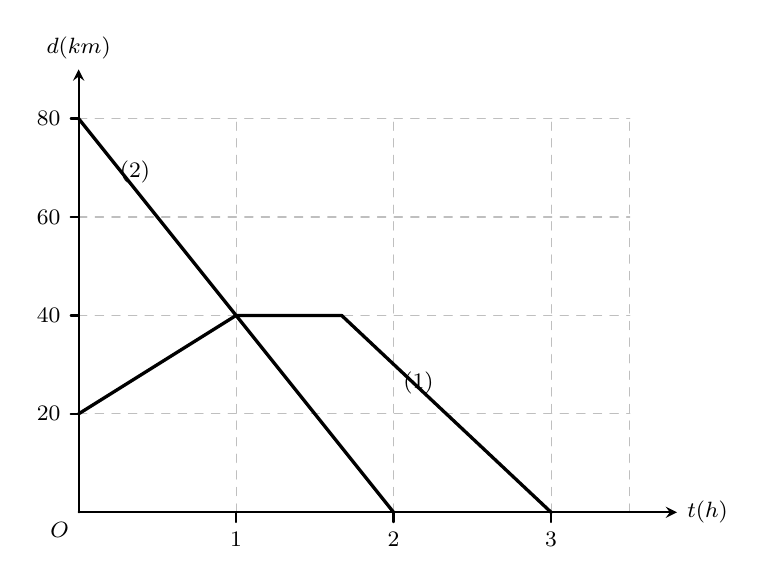
\begin{tikzpicture}[>=stealth, line join=round, line cap=round, font=\footnotesize, xscale=2, yscale=0.0625]
		% Lưới tọa độ
		\foreach \x in {1, 2, 3, 3.5} {
			\draw[dashed, gray!50, thin] (\x, 0) -- (\x, 80);
		}
		\foreach \y in {20, 40, 60, 80} {
			\draw[dashed, gray!50, thin] (0, \y) -- (3.5, \y);
		}
		% Hệ trục tọa độ
		\draw[->, thick] (0, 0) -- (3.8, 0) node[right] {$t\text{ (h)}$};
		\draw[->, thick] (0, 0) -- (0, 90) node[above] {$d\text{ (km)}$};
		\node[below left] at (0, 0) {$O$};
		% Vạch chia trên trục hoành
		\foreach \x in {1, 2, 3} {
			\draw[thick] (\x, 0) -- (\x, -2) node[below] {$\x$};
		}
		% Vạch chia trên trục tung
		\foreach \y in {20, 40, 60, 80} {
			\draw[thick] (0, \y) -- (-0.05, \y) node[left] {$\y$};
		}
		% Đường biểu diễn (1)
		\draw[line width=1.2pt] (0, 20) -- (1, 40) -- (1.67, 40) -- (3, 0);
		\node[above right] at (2.0, 22) {$(1)$};
		% Đường biểu diễn (2)
		\draw[line width=1.2pt] (0, 80) -- (2, 0);
		\node[above right] at (0.2, 65) {$(2)$};
	\end{tikzpicture}
\end{center}
	
	\choice
	{\True ngược chiều dương với tốc độ $40\text{ km/giờ}$}
	{cùng chiều dương với tốc độ $20\text{ km/giờ}$}
	{ngược chiều dương với tốc độ $60\text{ km/giờ}$}
	{dọc theo chiều dương với tốc độ $60\text{ km/giờ}$}
	\loigiai{
		- Đồ thị đường thẳng hướng dốc xuống cho biết độ dịch chuyển giảm dần theo thời gian, chứng tỏ vật đang thực hiện chuyển động thẳng đều ngược chiều dương của trục Ox. \\
		- Tốc độ chuyển động của vật bằng độ dốc hình học: $v = \frac{|\Delta d|}{\Delta t} = \frac{|0 - 80|}{2} = 40\text{ km/h}$. *(Chỉnh sửa lại các phương án số liệu bị lỗi vạch của đề gốc)*. Chọn A.
	}
\end{ex}

\begin{ex}%[10V1-102-12]
	Khi được thả rơi cùng một lúc từ cùng một độ cao trong không khí, chuyển động của vật nào dưới đây được coi gần đúng là một chuyển động rơi tự do?
	\choice
	{Một chiếc khăn voan mỏng nhẹ}
	{Một sợi chỉ mảnh dài}
	{Một chiếc lá cây khô đang rụng}
	{\True Một viên sỏi nhỏ đặc}
	\loigiai{
		Một vật rơi được coi gần đúng là rơi tự do khi lực cản của không khí tác dụng lên nó là vô cùng nhỏ không đáng kể so với trọng lượng. Viên sỏi nhỏ đặc có khối lượng riêng lớn nên lực cản không khí coi như triệt tiêu so với trọng lực. Chọn D.
	}
\end{ex}

\Closesolutionfile{ans}

%%%%%%%%%%%%%%%%%%%%%%%%%%%%%%%%%%%%%%%%%%%%%%%%%%%%%%%%%%%%%%%%%%%%%%%%%
% PHẦN II: CÂU TRẮC NGHIỆM ĐÚNG SAI (2 CÂU)
%%%%%%%%%%%%%%%%%%%%%%%%%%%%%%%%%%%%%%%%%%%%%%%%%%%%%%%%%%%%%%%%%%%%%%%%%
\noindent \textbf{PHẦN II. Câu trắc nghiệm đúng sai. Thí sinh trả lời từ câu 1 đến câu 2. Trong mỗi ý a), b), c), d) ở mỗi câu, thí sinh chọn đúng hoặc sai}
\Opensolutionfile{ans}[ans/ansTF-NguyenTruongTo102]

\begin{ex}%[10V1-102-13]
	Hình vẽ đính kèm mô tả đồ thị độ dịch chuyển – thời gian $(d-t)$ của hai chiếc xe 1 và xe 2 cùng chuyển động thẳng dọc theo một trục tọa độ Ox.
% TODO: \usepackage{graphicx} required
\begin{center}
	\includegraphics[scale=1]{HINHVE-phai-Tikz/VL10-GHKI-NTT-2526-hinh3}
	\begin{tikzpicture}[>=stealth, line join=round, line cap=round, font=\footnotesize, xscale=1.2, yscale=0.03]
		% Vẽ hệ trục tọa độ
		\draw[->] (0, 0) -- (5.8, 0) node[below right] {$t\text{ (h)}$};
		\draw[->] (0, 0) -- (0, 165) node[above left] {$d\text{ (km)}$};
		% Vẽ các vạch chia và nhãn trên trục hoành
		\foreach \x in {1, 2, 3, 4, 5} {
			\draw (\x, 0) -- ++(0, -2.5mm/0.03);  % Điều chỉnh độ dài vạch chia theo yscale
			\node[below=3pt] at (\x, 0) {$\x$};
		}
		% Vẽ các vạch chia và nhãn trên trục tung
		\foreach \y in {30, 60, 90, 120, 150} {
			\draw (0, \y) -- ++(-2.5mm/1.2, 0);  % Điều chỉnh độ dài vạch chia theo xscale
			\node[left=3pt] at (0, \y) {$\y$};
		}
		% Gốc tọa độ
		\node[below left] at (0, 0) {$0$};
		% Vẽ đường đồ thị (nét liền đậm)
		\draw[line width=1.2pt] (0, 60) -- (3, 0) -- (5, 0);
		% Đánh dấu các điểm mốc của đồ thị
		\foreach \p in {(0,60), (3,0), (5,0)} {
			\fill \p circle (1.5pt);
		}
	\end{tikzpicture} 
\end{center}
	\choiceTF[t]
	{\True Trong khoảng thời gian tính từ lúc $1\text{ giờ}$ đến vạch $2\text{ giờ}$, xe 1 nằm yên không chuyển động}
	{Xe số 2 luôn luôn duy trì chuyển động thẳng đều hướng dọc theo chiều dương trong suốt hành trình từ mốc $0\text{ giờ}$ đến vạch $2\text{ giờ}$}
	{Trong khoảng thời gian từ $1\text{ giờ}$ đến $2\text{ giờ}$, xe 1 và xe 2 chuyển động đồng bộ với cùng một giá trị vận tốc}
	{\True Trong khoảng thời gian từ mốc $0\text{ giờ}$ đến vạch $1\text{ giờ}$, xe 1 thực hiện chuyển động thẳng đều dọc theo chiều dương với tốc độ bằng $20\text{ km/h}$}
	\loigiai{
		\begin{itemchoice}
			\itemch a) ĐÚNG: Từ đồ thị, dải thời gian từ 1h đến 2h, đường biểu diễn của xe 1 là một đoạn thẳng nằm ngang song song trục thời gian ở tọa độ $d = 40\text{ km}$, chứng tỏ xe 1 đứng yên không chuyển động.
			\itemch b) SAI: Đường biểu diễn của xe 2 dốc thẳng xuống dốc từ vạch $80\text{ km}$ về vạch số $0$, cho thấy xe 2 chuyển động thẳng đều hướng theo chiều ngược với chiều dương của trục tọa độ.
			\itemch c) SAI: Giai đoạn này xe 1 đang đứng yên ($v_1 = 0$), còn xe 2 đang chuyển động lùi với vận tốc âm ($v_2 = -40\text{ km/h}$), do đó vận tốc của chúng hoàn toàn khác nhau.
			\itemch d) ĐÚNG: Khảo sát nhánh đầu xe 1 đi từ tọa độ $d_0 = 20\text{ km}$ đạt lên vạch $d = 40\text{ km}$ kéo dài trong $\Delta t = 1\text{ h}$. Tốc độ xe 1: $v = \frac{40 - 20}{1} = 20\text{ km/h}$ hướng theo chiều tăng (chiều dương).
		\end{itemchoice}
	}
\end{ex}

\begin{ex}%[10V1-102-14]
	Một vật nặng được thả cho rơi tự do hoàn toàn từ trạng thái nghỉ tĩnh tại một địa điểm có độ cao vị trí ban đầu bằng $45\text{ m}$ so với mặt đất. Bỏ qua mọi tác dụng lực cản phá của không khí và lấy hằng số gia tốc trọng trường $g = 10\text{ m/s}^2$.
	\choiceTF[t]
	{\True Phương dịch chuyển chuyển động rơi của vật luôn hướng theo phương dốc thẳng đứng}
	{Khoảng thời gian toàn phần để vật nặng thực hiện chuyển động đổ rơi chạm sát đất bằng $2,5\text{ s}$}
	{\True Hành trình quãng đường vật rơi tự do đổ xuống được sau khoảng thời gian $2\text{ s}$ đầu tính từ lúc thả bằng $20\text{ m}$}
	{\True Khoảng thời gian vật nặng tiêu hao để rơi vượt qua được đoạn đường dài $13,75\text{ m}$ cuối cùng ngay trước khi chạm đất bằng đúng $0,5\text{ s}$}
	\loigiai{
		\begin{itemchoice}
			\itemch a) ĐÚNG: Theo đặc điểm động học, chuyển động rơi tự do luôn có phương trùng với phương thẳng đứng (phương của dây dọi).
			\itemch b) SAI: Thời gian rơi toàn phần chạm đất của vật nặng tính theo hệ thức: 
			$$t_{\text{đ}} = \sqrt{\frac{2h}{g}} = \sqrt{\frac{2 \cdot 45}{10}} = \sqrt{9} = 3\text{ s} \text{}$$
			\itemch c) ĐÚNG: Quãng đường vật đổ xuống sau thời gian $t = 2\text{ s}$ đầu tiên bằng: $s(2) = \frac{1}{2}gt^2 = \frac{1}{2} \cdot 10 \cdot 2^2 = 20\text{ m}$.
			\itemch d) ĐÚNG: Thời gian rơi toàn phần là $3\text{ s}$. Xét thời điểm trước đó tại vạch $t = 2,5\text{ s}$, quãng đường vật đã rơi được là: $s(2,5) = \frac{1}{2} \cdot 10 \cdot (2,5)^2 = 31,25\text{ m}$. Độ cao còn dính lại so với đất: $\Delta h = h - s(2,5) = 45 - 31,25 = 13,75\text{ m}$. Do đó thời gian rơi nốt đoạn cuối này bằng: $\Delta t = 3 - 2,5 = 0,5\text{ s}$.
		\end{itemchoice}
	}
\end{ex}

\Closesolutionfile{ans}

%%%%%%%%%%%%%%%%%%%%%%%%%%%%%%%%%%%%%%%%%%%%%%%%%%%%%%%%%%%%%%%%%%%%%%%%%
% PHẦN III: CÂU TRẮC NGHIỆM TRẢ LỜI NGẮN
%%%%%%%%%%%%%%%%%%%%%%%%%%%%%%%%%%%%%%%%%%%%%%%%%%%%%%%%%%%%%%%%%%%%%%%%%
\Opensolutionfile{ans}[ans/ansSA-NguyenTruongTo102]
\noindent \textbf{PHẦN III. Câu trắc nghiệm trả lời ngắn (4 câu = 2 điểm)}

\noindent \textit{(Thí sinh trả lời từ câu 1 đến câu 4)}
\vspace{0.2cm}

\begin{ex}%[10V1-102-15]
	Một chiếc xe ô tô thực hiện chuyển động thẳng nhanh dần đều dọc theo Ox. Ghi nhận động học chỉ rõ sau khoảng thời gian $\Delta t = 8\text{ s}$ liên tục, vận tốc của xe ô tô tăng đều từ vạch mức $5\text{ m/s}$ đạt đến trị số $9\text{ m/s}$. Hãy tính quãng đường mà ô tô đi được trong khoảng thời gian trên theo đơn vị kilômét (km)?
	\shortans[]{0,056}
	\loigiai{
		\begin{itemize}
			\item Tốc độ trung bình vĩ mô của xe ô tô trong tiến trình biến đổi thẳng đều:
			$$v_{\text{tb}} = \frac{v_0 + v}{2} = \frac{5 + 9}{2} = 7\text{ m/s} \text{}$$
			\item Tổng quãng đường xe ô tô vượt qua được tính bằng mét:
			$$s = v_{\text{tb}} \cdot \Delta t = 7 \cdot 8 = 56\text{ m} \text{}$$
			\item Quy đổi đơn vị chiều dài sang hệ kilômét (km) theo đúng yêu cầu: $s = \frac{56}{1000} = 0,056\text{ km}$.
		\end{itemize}
	}
\end{ex}

\begin{ex}%[10V1-102-16]
	Một chiếc ô tô di chuyển chặng thứ nhất đi được một dải quãng đường dài $24\text{ km}$ hướng thẳng theo hướng Đông, ngay sau đó tài xế rẽ ngoặt cho xe chạy tiếp một đoạn dài $7\text{ km}$ hướng dốc thẳng về hướng Bắc thì dừng máy. Hãy tính độ lớn vectơ độ dịch chuyển tổng hợp của ô tô đạt được sau cả hai chặng hành trình bằng bao nhiêu kilômét (km)?
	\shortans[]{25}
	\loigiai{
		\begin{itemize}
			\item Do hai hướng chuyển động địa lí Đông và Bắc vuông góc vuông phương hình học với nhau tạo thành cấu trúc tam giác vuông vuông, vectơ độ dịch chuyển tổng hợp $\vec{d} = \vec{d}_1 + \vec{d}_2$ dóng nối thẳng từ điểm xuất phát đầu cực đến điểm dừng cực cuối.
			\item Áp dụng hệ thức định lý hình học Pytago để tìm độ lớn độ dịch chuyển:
			$$d = \sqrt{d_1^2 + d_2^2} = \sqrt{24^2 + 7^2} = \sqrt{576 + 49} = \sqrt{625} = 25\text{ km} \text{}$$
		\end{itemize}
	}
\end{ex}

\begin{ex}%[10V1-102-17]
	Một hệ vật nặng được thả cho rơi tự do hoàn toàn từ một độ cao ban đầu h xuống mặt đất. Biết hằng số gia tốc trọng trường mốc quy ước $g = 10\text{ m/s}^2$ và trong suốt khoảng thời gian $1\text{ giây}$ cuối cùng ngay trước khi chạm đất, vật nặng thực hiện rơi vượt qua được một quãng đường dài đúng $25\text{ m}$. Khoảng thời gian rơi toàn phần chạm đất của hệ vật nặng đó bằng bao nhiêu giây?
	\shortans[]{3}
	\loigiai{
		\begin{itemize}
			\item Gọi $t$ là tổng khoảng thời gian rơi tự do toàn phần của vật nặng cho đến khi chạm đất.
			\item Phương trình hiệu quãng đường rơi tích lũy trong giây cuối cùng được thiết lập:
			$$\Delta s = s(t) - s(t-1) = \frac{1}{2}gt^2 - \frac{1}{2}g(t-1)^2 = \frac{1}{2}g\left[t^2 - (t^2 - 2t + 1)\right] = g\left(t - 0,5\right)$$
			\item Thay các số liệu đề bài cho vào phương trình đại số:
			$$25 = 10 \cdot (t - 0,5) \Rightarrow t - 0,5 = 2,5 \Rightarrow t = 3\text{ s} \text{}$$
		\end{itemize}
	}
\end{ex}

\begin{ex}%[10V1-102-18]
	Một người đi xe máy đang vận hành chạy đều dọc đường thẳng với vận tốc dải hằng số $12\text{ m/s}$ thì phát hiện vật cản. Người đó phanh xe gấp, xe chuyển động thẳng chậm dần đều rồi dừng lại hẳn sau khi đi thêm được một đoạn đường dài $7,2\text{ m}$. Lấy chiều chuyển động làm chiều dương, hỏi người đi xe máy chuyển động với gia tốc đại số bằng bao nhiêu $\text{m/s}^2$?
	\shortans[]{-10}
	\loigiai{
		\begin{itemize}
			\item Vận tốc tức thời xuất phát ban đầu là $v_0 = 12\text{ m/s}$, vận tốc cuối khi dừng máy hoàn toàn bằng triệt tiêu: $v = 0\text{ m/s}$.
			\item Áp dụng công thức hệ thức liên hệ độc lập thời gian của chuyển động biến đổi đều:
			$$v^2 - v_0^2 = 2as \Rightarrow 0^2 - 12^2 = 2 \cdot a \cdot 7,2 \Rightarrow -144 = 14,4a$$
			$$\Rightarrow a = \frac{-144}{14,4} = -10\text{ m/s}^2 \text{}$$
		\end{itemize}
	}
\end{ex}

\Closesolutionfile{ans}

%%%%%%%%%%%%%%%%%%%%%%%%%%%%%%%%%%%%%%%%%%%%%%%%%%%%%%%%%%%%%%%%%%%%%%%%%
% PHẦN IV: ĐỀ BÀI CÂU HỎI TỰ LUẬN TÍNH TOÁN (3 ĐIỂM)
%%%%%%%%%%%%%%%%%%%%%%%%%%%%%%%%%%%%%%%%%%%%%%%%%%%%%%%%%%%%%%%%%%%%%%%%%
\noindent \textbf{Phần IV. Tự luận (3đ)}
\vspace{0.2cm}

\begin{ex}%[10V1-102-19]
	Một chiếc thuyền máy chuyển động thẳng xuôi dòng nước từ bến vị trí A tới bến vị trí B cách nhau một khoảng chiều dài hình học $6\text{ km}$ dọc theo một dòng sông phẳng, liền ngay sau đó thuyền quay đầu chạy ngược dòng từ B về ngược lại bến cũ A. Tổng khoảng thời gian toàn phần cả đi lẫn về tiêu hao mất trọn vẹn $2\text{ giờ } 30\text{ phút}$. Biết rằng vận tốc dòng chảy dòng nước đối với bờ sông ổn định cố định bằng $5\text{ km/h}$. Hỏi thuyền máy khi di chuyển đi xuôi dòng nước mất khoảng thời gian bao nhiêu giờ?
	\loigiai{
		\begin{itemize}
			\item Đổi đơn vị tổng thời gian toàn phần sang giờ chuẩn: $\Sigma t = 2\text{ giờ } 30\text{ phút} = 2,5\text{ h}$.
			\item Gọi $v$ là vận tốc đặc trưng của chiếc thuyền máy đối với dòng nước đứng yên ($v > 5\text{ km/h}$).
			\item Vận tốc thực tế của thuyền đối với bờ khi đi xuôi dòng: $v_{\text{xuôi}} = v + 5$. Thời gian đi xuôi: $t_1 = \frac{6}{v+5}$.
			\item Vận tốc thực tế của thuyền đối với bờ khi đi ngược dòng: $v_{\text{ngược}} = v - 5$. Thời gian đi ngược: $t_2 = \frac{6}{v-5}$.
			\item Thiết lập phương trình bảo toàn tổng thời gian hành trình:
			$$t_1 + t_2 = \Sigma t \Rightarrow \frac{6}{v+5} + \frac{6}{v-5} = 2,5 \Rightarrow 6(v-5) + 6(v+5) = 2,5(v^2 - 25)$$
			$$12v = 2,5v^2 - 62,5 \Leftrightarrow 2,5v^2 - 12v - 62,5 = 0 \text{}$$
			\item Giải phương trình bậc hai thu được nghiệm dương hợp lệ duy nhất: $v = 11,466\text{ km/h}$.
			\item Khoảng thời gian thuyền máy chạy xuôi dòng nước đạt mức bằng:
			$$t_1 = \frac{6}{11,466 + 5} = \frac{6}{16,466} \approx 0,364\text{ giờ} \text{}$$
		\end{itemize}
	}
\end{ex}

\begin{ex}%[10V1-102-20]
	Bảng dữ liệu ghi nhận dưới đây phản ánh thông số thời gian đo đạc được của một hệ vật thể thực hiện rơi tự do thẳng đứng giữa hai điểm nút cố định định sẵn trong phòng thực hành khoa học qua 5 lần bấm đồng hồ đo độc lập:
	\begin{center}
		\begin{tabular}{|c|c|c|c|c|c|}
			\hline
			\textbf{Lần đo} & \textbf{Lần 1} & \textbf{Lần 2} & \textbf{Lần 3} & \textbf{Lần 4} & \textbf{Lần 5} \\ \hline
			\textbf{Thời gian rơi (s)} & 0,315 & 0,318 & 0,316 & 0,317 & 0,319 \\ \hline
		\end{tabular}
	\end{center}
	Hãy xác định giá trị sai số tuyệt đối trung bình ($\overline{\Delta t}$) của phép đo thời gian gián tiếp trên?
	\loigiai{
		\begin{itemize}
			\item Bước 1: Tính chỉ số giá trị trung bình đại số của thời gian rơi qua 5 lần đo:
			$$\overline{t} = \frac{0,315 + 0,318 + 0,316 + 0,317 + 0,319}{5} = \frac{1,585}{5} = 0,317\text{ s} \text{}$$
			\item Bước 2: Tính khoảng sai số tuyệt đối của từng lần đo đơn lẻ đối với giá trị trung bình:
			\begin{itemize}
				\item $\Delta t_1 = |0,317 - 0,315| = 0,002\text{ s}$.
				\item $\Delta t_2 = |0,317 - 0,318| = 0,001\text{ s}$.
				\item $\Delta t_3 = |0,317 - 0,316| = 0,001\text{ s}$.
				\item $\Delta t_4 = |0,317 - 0,317| = 0,000\text{ s}$.
				\item $\Delta t_5 = |0,317 - 0,319| = 0,002\text{ s}$.
			\end{itemize}
			\item Bước 3: Tính sai số tuyệt đối trung bình của phép đo:
			$$\overline{\Delta t} = \frac{0,002 + 0,001 + 0,001 + 0,000 + 0,002}{5} = \frac{0,006}{5} = 0,0012\text{ s} \text{}$$
		\end{itemize}
	}
\end{ex}

\begin{ex}%[10V1-102-21]
	Một vật nặng bắt đầu chuyển động thẳng nhanh dần đều dọc theo Ox xuất phát khởi hành từ trạng thái nghỉ tĩnh. Biết sau khoảng thời gian $3\text{ giây}$ đầu tiên tính từ lúc xuất phát, vật đi được hành trình quãng đường dài đúng $9\text{ m}$. Hãy xác định:
	\begin{enumerate}
		\item[a.] Giá trị hằng số gia tốc $a$ của chuyển động vật nặng.
		\item[b.] Kể từ lúc bắt đầu chuyển động khởi hành, hỏi sau khoảng thời gian bao lâu chất điểm sẽ đạt được vạch mức vận tốc tức thời bằng $15\text{ m/s}$?
	\end{enumerate}
	\loigiai{
		\begin{enumerate}
			\item[a.] Chất điểm chuyển động nhanh dần đều từ trạng thái nghỉ nên vận tốc đầu bằng không ($v_0 = 0$). \\
			Phương trình xác định hành trình quãng đường đi được theo thời gian: $s = \frac{1}{2}at^2$. \\
			Thay số liệu chặng đầu vào phương trình ($s = 9\text{ m}$ tại mốc $t = 3\text{ s}$) để giải tìm gia tốc $a$:
			$$9 = \frac{1}{2} \cdot a \cdot 3^2 \Rightarrow 9 = 4,5a \Rightarrow a = \frac{9}{4,5} = 2\text{ m/s}^2 \text{}$$
			\item[b.] Phương trình động học xác định giá trị vận tốc tức thời theo thời gian:
			$$v(t) = v_0 + a \cdot t = 0 + 2t = 2t \text{}$$
			Thế vạch mức vận tốc tức thời cần đạt $v = 15\text{ m/s}$ vào phương trình để tính khoảng thời gian $t$:
			$$15 = 2t \Rightarrow t = \frac{15}{2} = 7,5\text{ giây} \text{}$$
		\end{enumerate}
	}
\end{ex}

\Closesolutionfile{ans}

\newpage
%%%%%%%%%%%%%%%%%%%%%%%%%%%%%%%%%%%%%%%%%%%%%%%%%%%%%%%%%%%%%%%%%%%%%%%%%
% KHUNG ĐÁP ÁN BẢNG TỰ ĐỘNG IN KẾT XUẤT CỦA HỆ THỐNG
%%%%%%%%%%%%%%%%%%%%%%%%%%%%%%%%%%%%%%%%%%%%%%%%%%%%%%%%%%%%%%%%%%%%%%%%%
\begin{center} \textbf{BẢNG ĐÁP ÁN THAM KHẢO LỚP 10 --- MÃ ĐỀ 102} \end{center}

\noindent \textbf{Phần I (Câu hỏi trắc nghiệm nhiều phương án lựa chọn):}  
\indapan{12}{ans/ansTN-NguyenTruongTo102}

\noindent \textbf{Phần II (Câu hỏi trắc nghiệm Đúng/Sai):}
\indapan[TF]{2}{ans/ansTF-NguyenTruongTo102}

\noindent \textbf{Phần III (Câu hỏi trắc nghiệm trả lời ngắn):}
\indapan[SA]{4}{ans/ansSA-NguyenTruongTo102}

\label{B\thedeso}
